\chapter{Summary of Research on Association}
	\label{cha:sum_association}
	
	This part of the thesis discussed the machine intuition process of association: the act of extracting important latent features from the data, in order to find meaningful similarities, through which individual observations can be assigned to- and processed as discrete groups.
	Among \ac{ML} algorithms, simpler statistical clustering algorithms approach this task in multiple ways.
	Centroid-based clustering (quantization) algorithms -- such as \kmeans{} or \ac{GMM} -- assume the final distribution of the data is made up of multiple Gaussians, and try to fit these iteratively through expectation-maximization.
	Density-based clustering algorithms -- such as \ac{DBSCAN} or \ac{OPTICS} \cite{dbscan, optics} -- traverse the data from one individual observation to the next, defining clusters as a group where the observations are reachable from each other, according to a certain distance threshold.
	\ac{HAC} merges individual observations, and later smaller clusters, into ever bigger clusters, finally arriving at a single cluster that encompasses the whole dataset.
	The hierarchy is represented as a tree (dendogram), where the clusters are defined by a user-set threshold of maximum distance, which splits the tree at a certain height.
	
	\begin{figure}[ht]
		\centering
		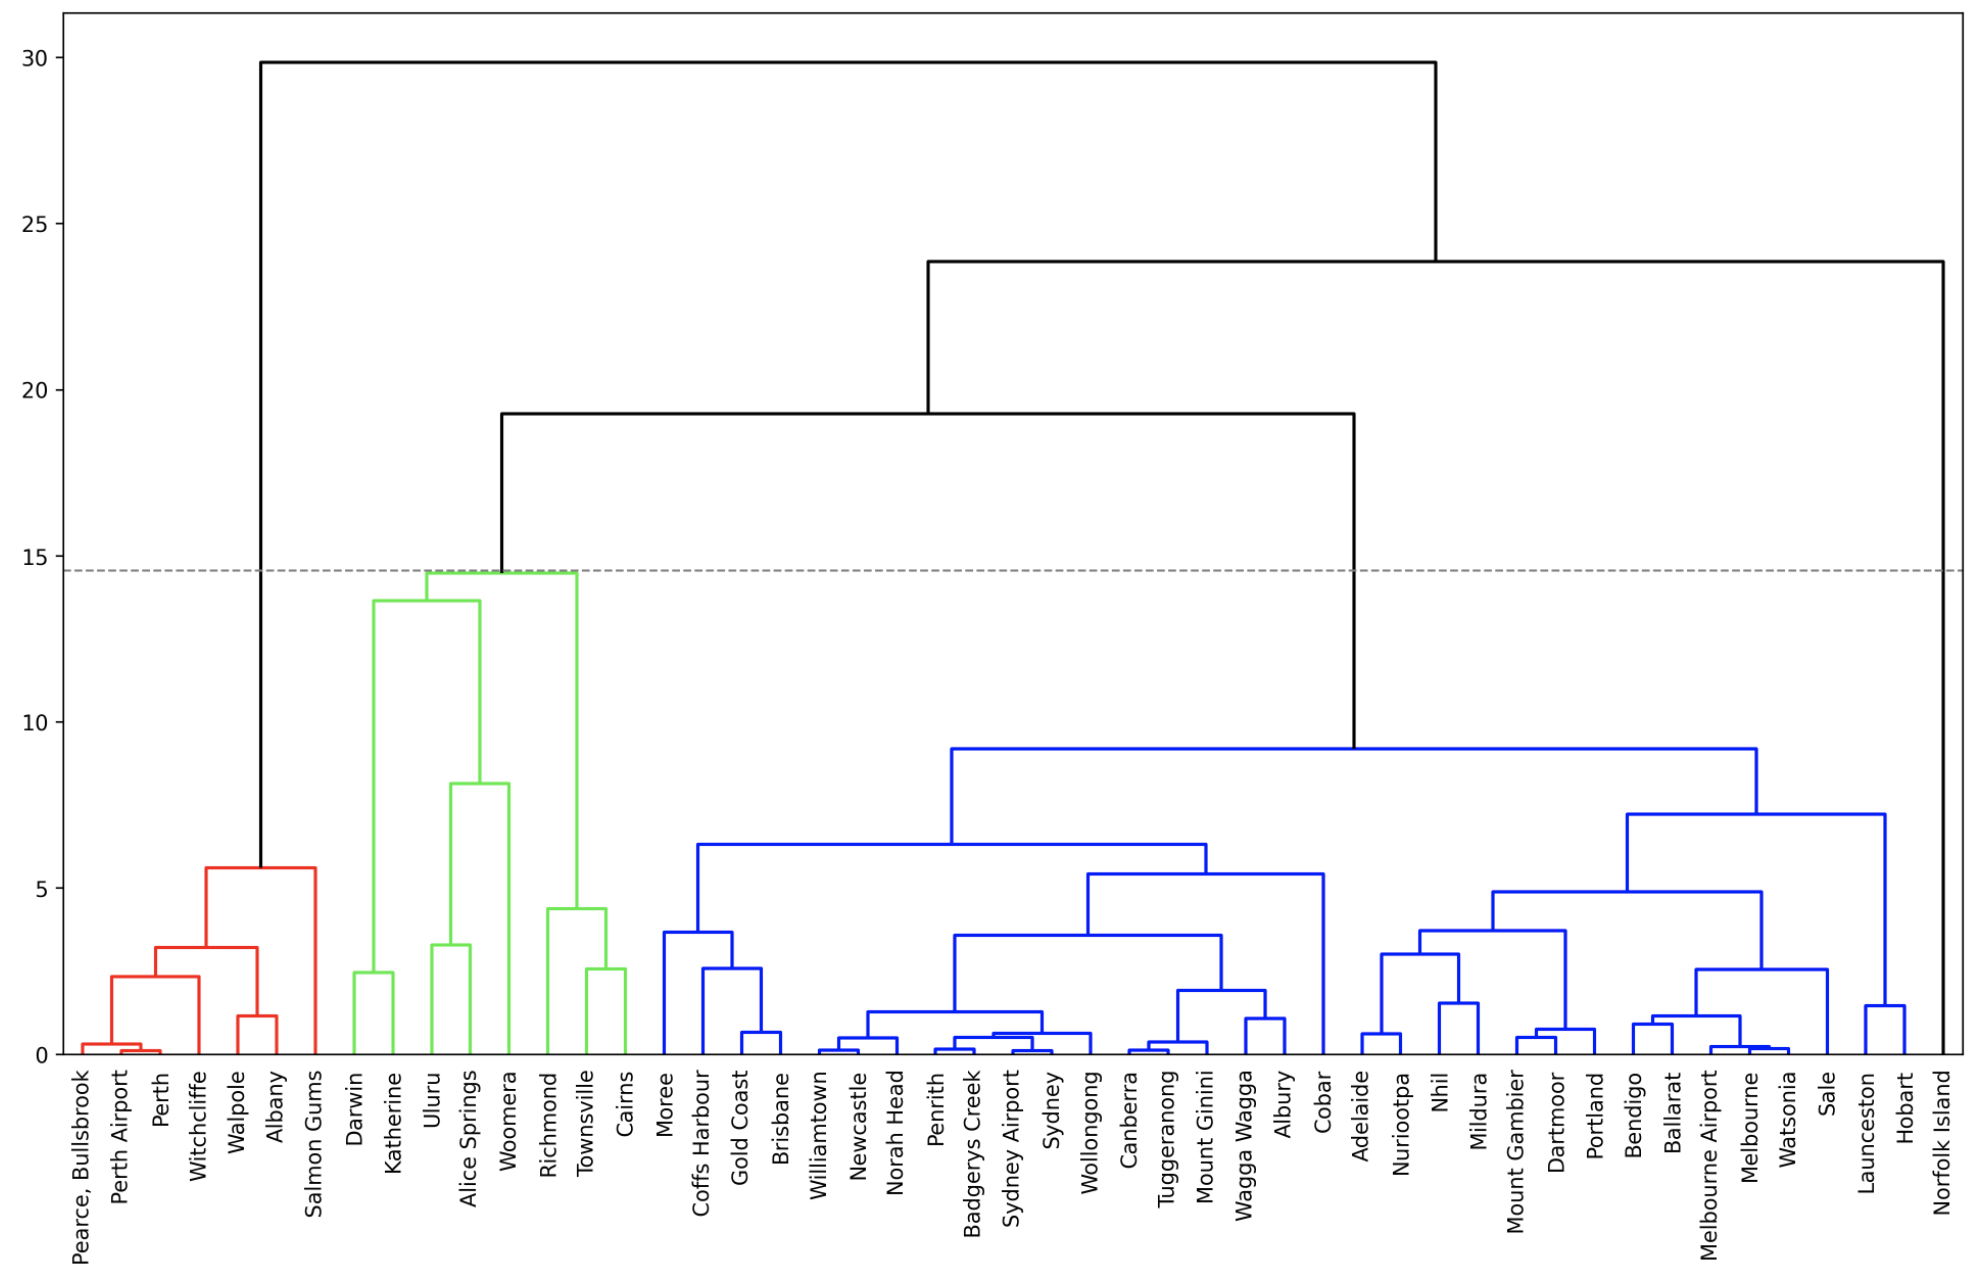
\includegraphics[width=0.5\linewidth]{figures/08_sum_association/hac/hac.png}
		\caption[HAC dendogram illustration]{A dendogram of larger cities in Australia formed by HAC.}
		\label{fig:hac}
	\end{figure}
	
	As all of the above mentioned clustering algorithms depend on some sort of distance metric, they all suffer from the \emphix{curse of dimensionality}{curse of dimensionality} when employed on data that contains many features.
	In this case, the curse of dimensionality manifests as the breakdown of distance metrics in high-dimensional space: in many dimensions, datapoints are likely to be close to the ``corners'' of the imaginary hypercube that encompasses them, virtually limiting the possible distances between datapoints to (a handful of) discrete values, which makes distance metrics less and less useful for defining clusters.
	These algorithms are also sensitive to the quality of input features.
	Features which contain irrelevant, or noisy data can obfuscate meaningful distance between the datapoints where without them, clusters could have been differentiated.
	Redundant features only add to the number of dimensions without adding useful information, once again worsening the effect of the curse of dimensionality.	
	Deep clustering algorithms overcome these limitations by encoding the data into a lower-dimensional space, extracting the latent features that govern the data and are meaningful for clustering.
	Furthermore, using additional constraints, deep clustering algorithms can also create a ``clustering-friendly'' encoding, in which similar observations are close to each other, while dissimilar observations are far apart, so that distance-based clustering algorithms work well with these representations.
	Indeed, this is the approach of many of the state-of-the-art deep clustering algorithms, which employ a deep neural net to form the latent encoding, and a secondary, statistical clustering step, which uses the encoded datapoints to from clusters.
	
	The first clustering algorithm discussed in this part, \ac{SCA}, is different to this common two-step approach.
	\ac{SCA} does not have a separate encoding and clustering step, instead, the encoding is constrained to map the datapoints to a specific structure (a simplex) in the latent space, which can be easily equated to a fully-connected graph.
	Because of the ample modeling capacity in deep neural nets, we reasoned that the encoding should be able to map datapoints in a clustering-friendly way even with this added constraint.
	Furthermore, the constraint used on the latent representation allows for datapoints to fall between the graph nodes (the simplex vertices).
	These in-between datapoints can be used to select which graph nodes have connecting edges (simplex edges), and which do not, according to a user-set edge-population value.
	Through the connecting edges, \ac{SCA} has an almost agglomerative approach to clustering, where clusters are formed by graph nodes that are reachable from each other.
	This approach alleviates a common downside of many clustering algorithms: having to define the number of clusters ($k$) before the algorithm is run.
	
	An important side-effect of the graph-like representation is the explainability of the model.
	During the design, we specifically wanted to create an algorithm that represents mobile network data as a ``state transition graph'': a quantized model, where the network or individual elements are either in a state, or are transitioning between two states.
	The states were meant to be granular enough so that they can be represented by a single prototype observation, which is the core idea of quantization.
	We argued that such a representation is easy to understand for us humans, as our thinking naturally tends towards such models, and is also present in other commonly used \ac{ML} models, such as Markov chains.
	Furthermore, we believed this explainability would carry over to other \ac{ML} tasks that are undertaken using the state transition graph representation.
	
	\ac{SCA} was evaluated on the task of cell anomaly detection, where, with the help of the state transition graph, it is possible to define $3$ explainable cell anomaly types: anomalous states, static, and dynamic anomalies.
	Our evaluation focused on the detection of anomalous states, however, as we unfortunately lacked a dataset that contains labeled cell anomalies, we were unable to provide a quantitative evaluation, and had to resort to a more qualitative demonstration of the benefits of using \ac{SCA}.
	In order to try to provide a quantitative comparison to other clustering algorithms, we evaluated \ac{SCA} on a common image dataset.
	Unfortunately, we were unable to achieve consistently good results, as the sparsity constraint would often force points from two or more classes into the same quantum.
	These impure quanta drastically limit the clustering accuracy, even if not all quanta are mixed.
	In the end, it seems our hypothesis was incorrect, as the added constraint of the simplex often overtly disturbs the encoder, which in turn does not produce a coherent latent encoding, mixing datapoints from different clusters together only to adhere to the constraint.
	Overall, the problem with \ac{SCA} is rooted in the common fallacy of extensive human bias during the design of the algorithm.
	By wanting to have an explainable model, we have enforced an internal representation/interface on the algorithm that is not useful for machine learning.
	
	While trying to improve our \ac{SCA} algorithm, we evaluated a handful of image clustering algorithms on mobile network data.
	These algorithms often didn't perform as well on mobile data as they did on their originally intended data type, which we suspected was caused by two aspects of our datasets: first, a large portion of the logged \acp{KPI} in our datasets contained clustering-irrelevant features, and second, the data did not behave as images, so many of the preconceptions which apply to that domain did not apply to ours.
	This motivated us to try to develop a clustering algorithm, which has a reliable performance on mobile network data that is on par with state-of-the-art image clustering performance.
	Learning from the mistakes in \ac{SCA}'s design, we developed a deep clustering algorithm called \ac{DANCE}.
	Instead of the single-step design of \ac{SCA}, \ac{DANCE} is a multi-step clustering algorithm, utilizing a simpler secondary clustering algorithm for the initial formulation of the clusters.
	Furthermore, while \ac{DANCE} also poses restrictions on the internal representation to make it clustering-friendly, this restriction is more forgiving, allowing for other, non-clustering-friendly information to also propagate in the model.
	This is the main feature of \ac{DANCE}, where the clustering-relevant features are isolated from the clustering-irrelevant ones, which is achieved through the decorrelation of latent features separated into two groups.
	Through this mechanism, \ac{DANCE} is able to reduce and refine the feature-set used for the later clustering steps, achieving reliably good performance that surpasses other state-of-the-art algorithm's performance by a sizable margin on mobile network data.
	
	% Clustering:
	% * Is it a feasible concept technically?
	%   -> Yes, we have seen the algorithms, however, requires a lot of expertise to define/use, design bias might overwhelm the results.
	% * Is clustering in mobile network automation beneficial?
	%   -> Not in itself, because the same could be undertaken with classification. It could be, however, very useful as augmentation for data generation/labeling process.
	% * Is it a feasible concept in terms of complexity, runtime?
	%   -> Yes, if trained offline, and only used for inference, but if regularly trained, no. The connected encoding-clustering nature makes it slow and heavy.	
	
	\section{Assessment of Feasibility (A2.1)}
	
		Associative modeling can potentially be realized to a high precision with deep clustering using neural nets.
		The neural nets preprocess the data before the cluster formulation, by extracting relevant features and reducing the dimensionality of the data, as well as encoding it in a clustering-friendly way, allowing simpler clustering algorithms to find latent classes which are not explicitly defined in the data.
		Usually, the task of clustering in general and the deep neural nets used specifically means a sizable dataset is required for good precision.
				
		Clustering algorithms, among other similarities, often share the need of a predefined number of clusters $k$ with quantization algorithms.
		However, in the clustering case, the $k$ parameter is not so forgiving: an incorrect setting of $k$ means either some clusters have to include more than one ground truth class, or a single class has to be divided between multiple clusters, making an accurate clustering impossible from the start.
		Clustering in general requires a lot of domain specific knowledge from the user, in order to set the parameters of the algorithms correctly, most prominently required in the tuning of the parameters that govern the additional restrictions for the encoding.
		Insufficient domain knowledge can lead to incorrect bias in these parameters, which has a strong impact on the precision of these algorithms.
		Furthermore, clustering algorithms also require a great deal of \ac{DL} expertise of the user, such as when defining the neural net topologies or balancing the losses during training.
		A lack of this expertise can also easily lead to lowered precision, because of under- or overtraining, or improperly balanced losses.
		Finally, design-time bias can be present in the algorithms that makes them inapplicable to the mobile networks domain, as we have seen with some image clustering algorithms.

	\section{Assessment of Practicality (A2.2)}
	
		Feature extraction done by an encoding step can greatly reduce the number of dimensions the secondary clustering algorithms have to work with, thereby lessening the scaling of runtime/computational requirements with the data dimensions, as well as making them robust against the curse of dimensionality.
		However, as the encoding is mostly done with deep neural nets, the encoding step itself is usually quite computationally heavy.
		For inference -- when the deep clustering algorithm is only used for assigning new observations to previously established clusters -- \ac{DL}-based clustering algorithms are relatively quick.
		However, if clustering is used as a ``whole'' (i.e.: discovering new clusters), training \ac{DL}-based clustering algorithms can take an exorbitant amount of time, which impacts their usefulness.
		Accompanying these large computational requirements are large memory consumption and data volume need, which in turn translates to a significant cost in storage and possibly data transfer.
		These requirements basically exclude deep clustering to be used on constrained devices with limited storage, memory, computational or power capacity, such as mobile devices.
		
		On the one hand, for now, there are not many applications where these algorithms are meant to be repeatedly retrained.
		One such example is cell anomaly detection, where the models are usually meant to be periodically retrained in order to allow them to follow slow changing contexts.
		In most other cases, the clustering algorithms are meant to be trained offline and only once, which generally can take a long time without impact.
		On the other hand, a shorter training duration and lighter requirements could open up use cases in the future that are currently not considered, because of the extensive resource needs of these algorithms.
				
	\section{Assessment of Applicability (A2.3)}
	
		The use of clustering makes sense for problems where there are certainly different types (classes) in the data, such as user behavior/usage-related modeling, or discrete (state-) logic in the network, such as network slicing.
		In data that does not have latent classes, deep clustering will not do more than what simpler quantization algorithms already do: splitting up a continuous range of variation into arbitrary discrete clusters.
		However, that does not diminish their utility over simpler quantization algorithms: we have seen how important it is for quantization algorithms to align quanta with class boundaries, if such classes are indeed present in the data.	
		Clustering techniques are ``backwards'' applicable to these problems, where a clustering friendly encoding can help the quantization algorithm in the aligned definition of the quanta.
		
		Deep clustering training requires a lot of context-specific bias -- as we have seen when using algorithms on mobile network data meant for image-recognition -- which might mean that even if the algorithm is applicable to one mobile network context, it might not be portable between different contexts, such as different locations, vendors, operators, or different generations.
		Thus, deep clustering algorithms are very context-specific (i.e.: not reusable), and probably need to be trained and fine-tuned not only for use cases, but for individual uses.
		
		The above restrictions limit the applicability of deep clustering in mobile networks, and make their use questionable even in the few use cases which do have inherent classes and allow for context-specific deployments.
		The strong need for human supervision in these algorithms counteracts our original goal with the use of unsupervised learning: the reduction of human labor.
		In my opinion, even if a problem does warrant the use of deep clustering, most of the time it is better solved by supervised classification algorithms instead.
		Classification generally has higher precision than clustering if applied on the same problem, usually with a much simpler model (shallower neural net), speeding up training and inference, as well as greatly reducing memory and power consumption, possibly allowing for the use of deep classification even on mobile devices.
		Since clustering algorithms also seem to require context-specific tuning, the need for a labeled dataset does not necessarily mean a larger need for human labor compared to clustering algorithms, more of a shift in what type of labor the expert has to do.		
	
		However, all is not lost for deep clustering algorithms. 
		Because of the complexity of mobile network data, the use of deep clustering algorithms is often warranted for the purpose of reducing the amount of observations that need to be manually labeled for supervised classification algorithms.
		In this role, clustering algorithms are a supporting tool in the hands of the mobile networks expert: by initially labeling a few key observations manually, the expert can tune the clustering parameters to best align the clusters with the initial labels.
		After this, by labeling whole clusters, the clustering algorithm can be used to produce labeled observations for the training of a classification algorithm.
		In this workflow, deep clustering is both a data-exploratory and a data-preprocessing tool, helping in the development and deployment of simpler, lightweight classification models.	